\chapter{Entanglement}

%\begin{abstract}

In this chapter, we will finally learn about \emph{entanglement}: a special, very unique feature of quantum mechanics. We will begin by demonstrating how strange entanglement can be and how counter-intuitive it can be. Then we will move on to the definition of what entangled states are, and then we will talk about a particular class of entangled states called "Bell states", which play a very important role in quantum communication and quantum computation. Finally, we will finish by framing entanglement as a resource for computational and communication tasks.

%\end{abstract}

\section{CHSH Game}
\label{sec:chsh-game}
\index{CHSH game}

\if0
% table of possibilities
\begin{figure}[H]
    \centering
    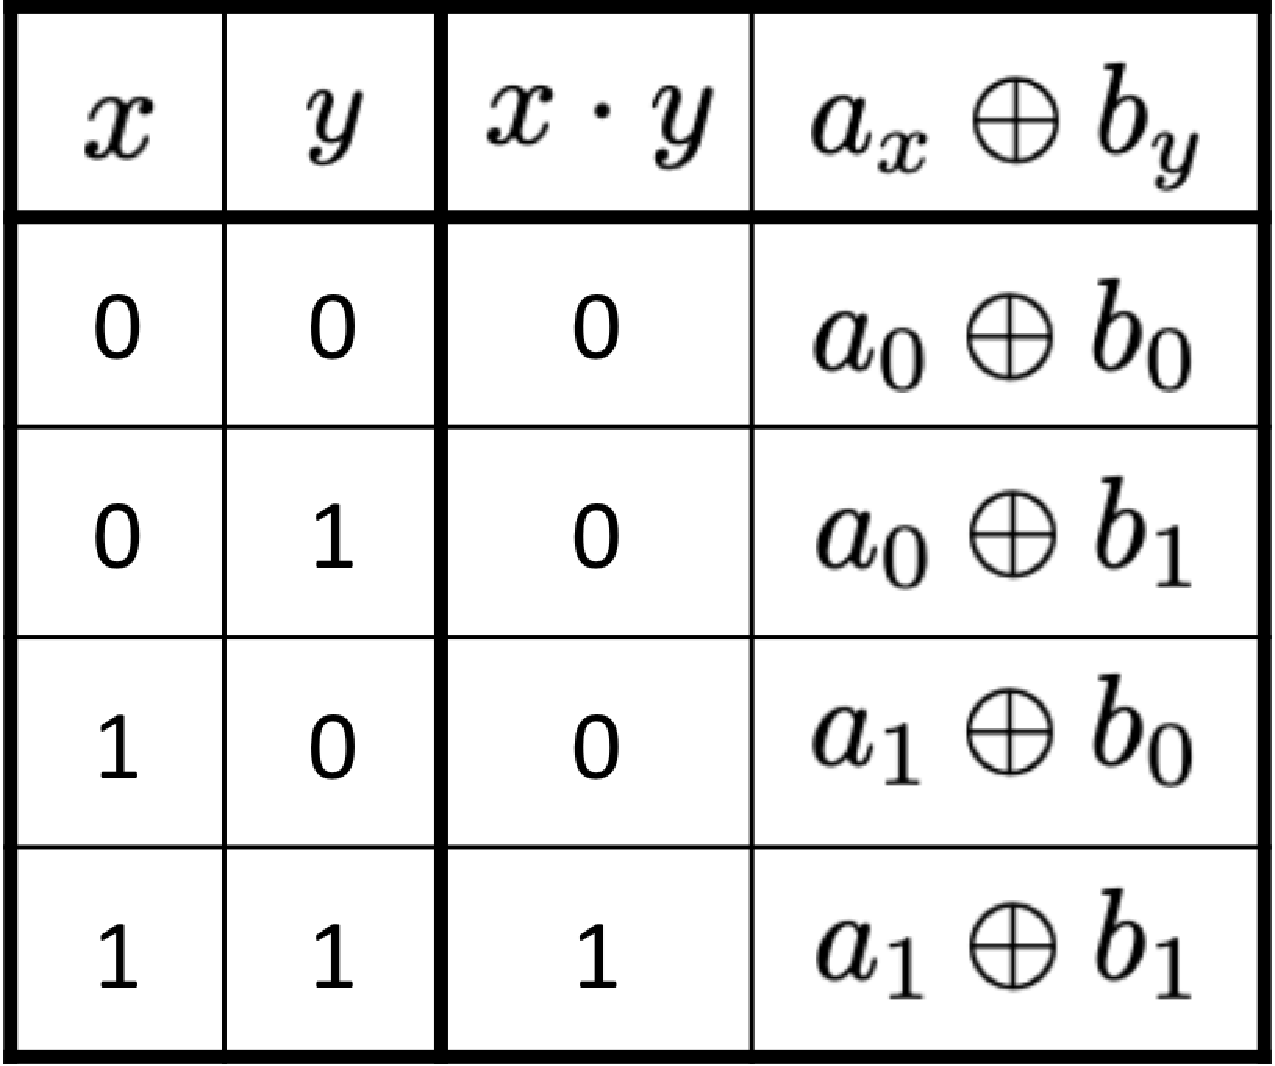
\includegraphics[width=0.8\textwidth]{lesson4/CHSH_table.pdf}
    \label{fig: 1}
    
        \caption{CHSH game}
    
\end{figure}
\fi

% Lesson Four: Entanglement.


% Step One: CHSH Game.

We will begin with a game, and the rules of the game are the following: Players "A" and "B" are trying to cooperate to win a game that's being refereed by another person, whom we will call "R".

% game diagram
\begin{figure}[H]
    \centering
    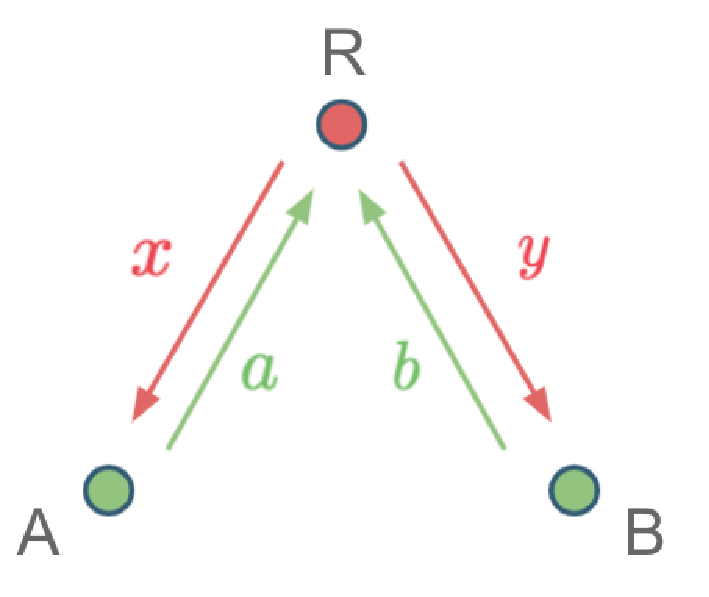
\includegraphics[width=0.5\textwidth]{lesson4/CHSH_diagram.pdf}
        \caption[CHSH game view]{CHSH game view. The players A and B attempt to collaborate to beat the referee R.}
    \label{fig:chsh-game}
\end{figure}

The game, as shown in Fig.~\ref{fig:chsh-game}, begins with R generating two classical bits $x$ and $y$, fully at random, and sending the $x$ bit to player A and the $y$ bit to player B. Then the players A and B reply with their own classical bits $a$ and $b$. They win one round of the game if the product $xy$ is equal to the binary sum $a + b$. But there is one very important constraint: once the game begins, players A and B are not allowed to communicate. You see, if they could communicate, A could just tell B: hey, the bit $x$ I received is equal to zero or is equal to one, and they could very easily win every round.

But this doesn't mean that they are not cooperating. Before the game begins, they can actually decide on their strategy, or what bits and in what fashion they will output. Let's have a look how this actually works in practice, as shown in Fig.~\ref{fig:chsh-game-rounds}. Let's say, for example, that $x =0$, $y = 1$. That means that the product zero times one is just zero. A replies with its bit, which is zero, and B replies with a one, and the binary sum $a + b = 0 + 1 = 1$. We see that the product zero and sum one are not equal, therefore the players A and B lose this particular round.
% Round 1/2/3 pic
\begin{figure}[H]
    \centering
    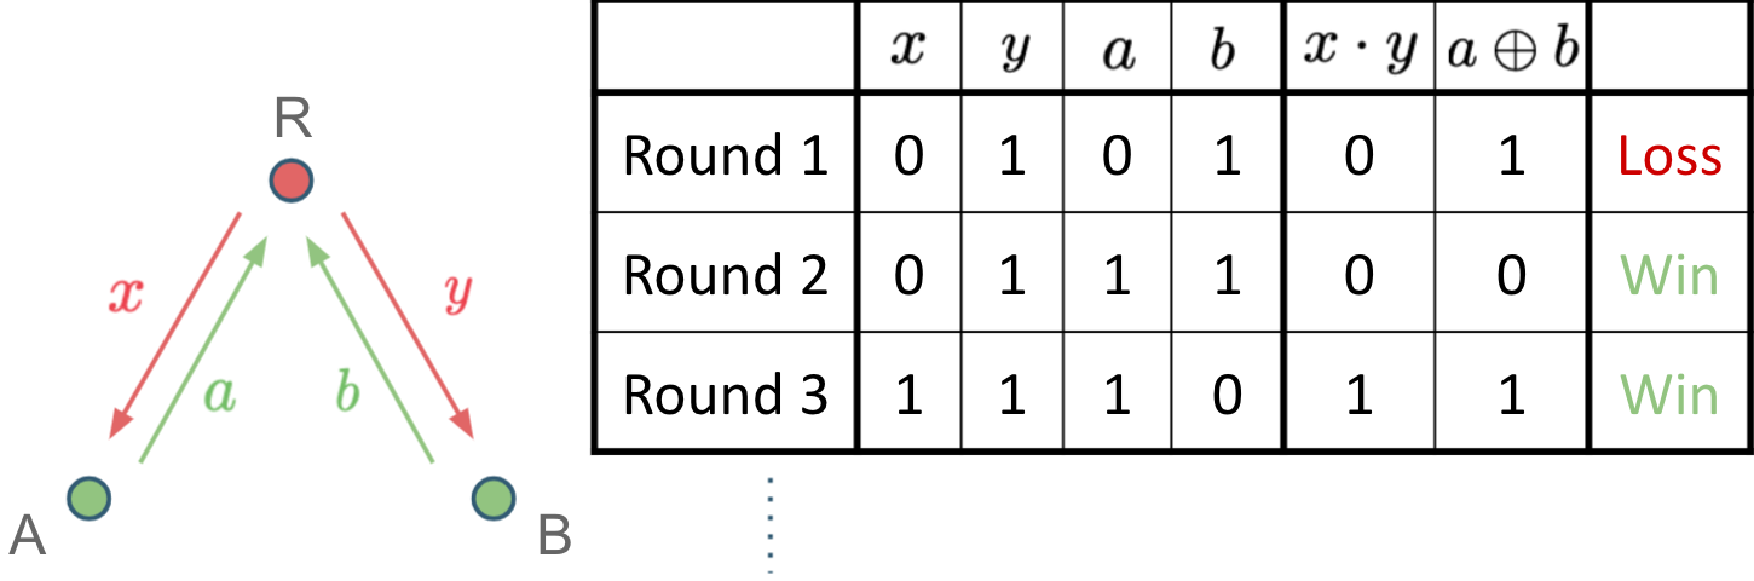
\includegraphics[width=0.8\textwidth]{lesson4/CHSH_rounds.pdf}
        \caption{Three rounds of the CHSH game.}
    \label{fig:chsh-game-rounds}
\end{figure}

In the next round, maybe $x$ and $y$ are still zero and one, but this time $a = b = 1$. Now the binary sum $a + b = 1 + 1 = 0$. So we see that they satisfy the winning condition: $xy$ is equal to $a + b$, therefore they win. In round three, maybe the $x$ and $y$ actually change. They're both one, and A and B reply with one and zero, respectively. In this case we can see again that they win because the product of $x$ and $y$ is equal to the binary sum of $a$ and $b$. They keep going on and on like this, repeating the game. But the main question is: what strategy should A and B follow in order to maximize the win rate? Of course they could just randomly generate their bits and be satisfied that sometimes they win and sometimes they lose, but our players are actually competitive and they try to win every single round, so let's see if that's actually possible.

% insert annotated table of possibilities
\begin{figure}[H]
    \centering
    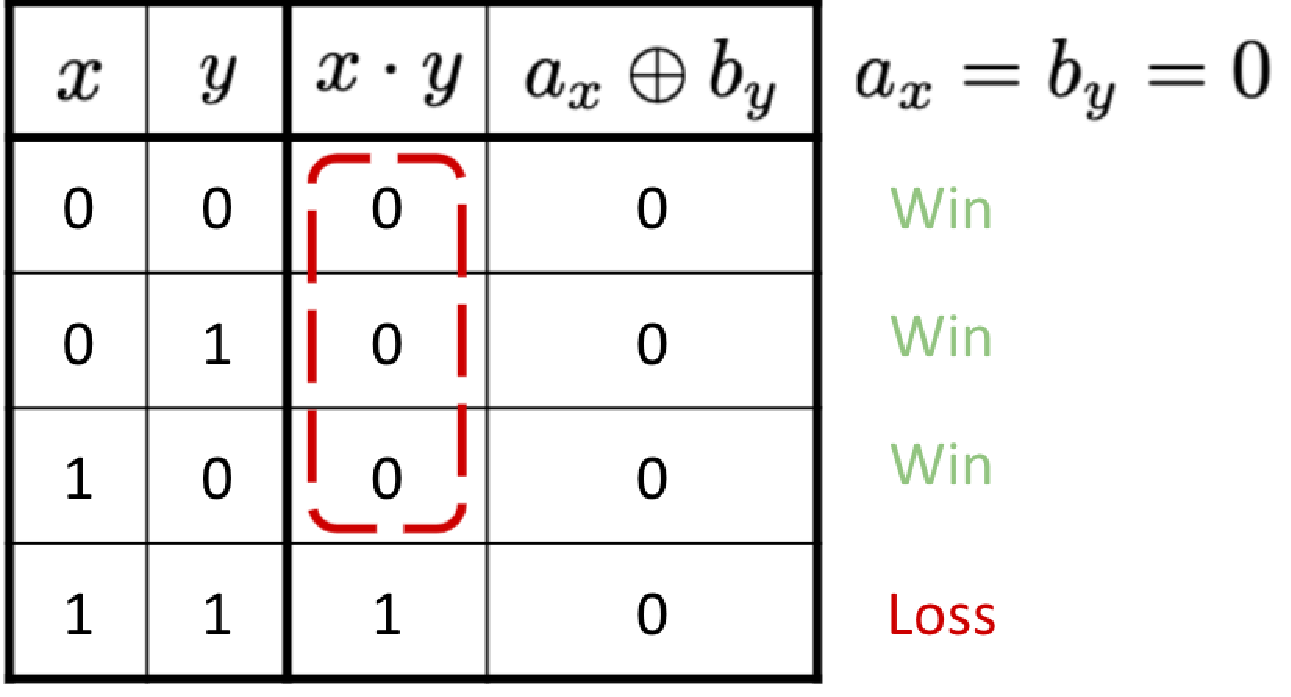
\includegraphics[width=0.8\textwidth]{lesson4/CHSH_annotated_table.pdf}
        \caption[CHSH game and outcomes]{CHSH game and outcomes for the four possible $x, y$ values, when A and B both have chosen zero for their secret bits.}
    \label{fig:chsh-table}
\end{figure}

The table shown in Fig.~\ref{fig:chsh-table} lists all four possible bit pairs that the referee can distribute to A and B, (0, 0), (0, 1), (1, 0), and (1, 1). The third column lists the $x\cdot y$ products that A and B are attempting to match. As an example, this figure assumes that A and B chose $a_x = b_y = 0$, and shows that their value $a_x \oplus b_y$. We are calling them $a_x$ and $b_y$ to emphasize that the output bits $a$ and $b$ can be chosen depending on the bits $x$ and $y$ that the players received from the referee. You can try and substitute any values for $a_x$ and $b_y$, and in fact you will see that they cannot satisfy the winning condition all the time. It's just inevitable that in some cases they will lose.

In the first three cases, the product of $x$ and $y$ is zero. It's only in the last case when it's one. In fact, A and B can just say, "o matter what $x$ and no matter what $y$ we received, we will always reply with the output zero." That is one viable strategy. So $a$ is always zero, $b$ is always zero, and in that case they win the game three out of four times. You can be a little bit more mathematical and can prove that even in fact if they follow any other strategy, they cannot go higher than this 75 percent win rate. 


% insert quantum diagram
\begin{figure}[H]
    \centering
    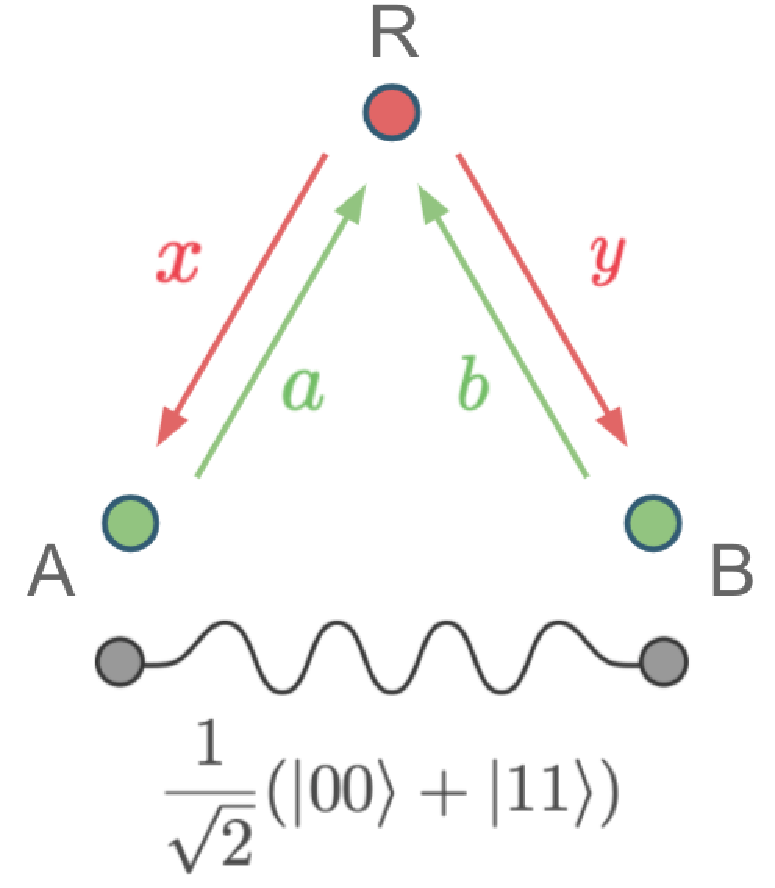
\includegraphics[width=0.5\textwidth]{lesson4/CHSH_quantum_diagram.pdf}
        \caption{Quantum version}
    \label{fig:chsh-quantum}
\end{figure}

% Quantum まとめ guide
\begin{figure}[H]
    \centering
    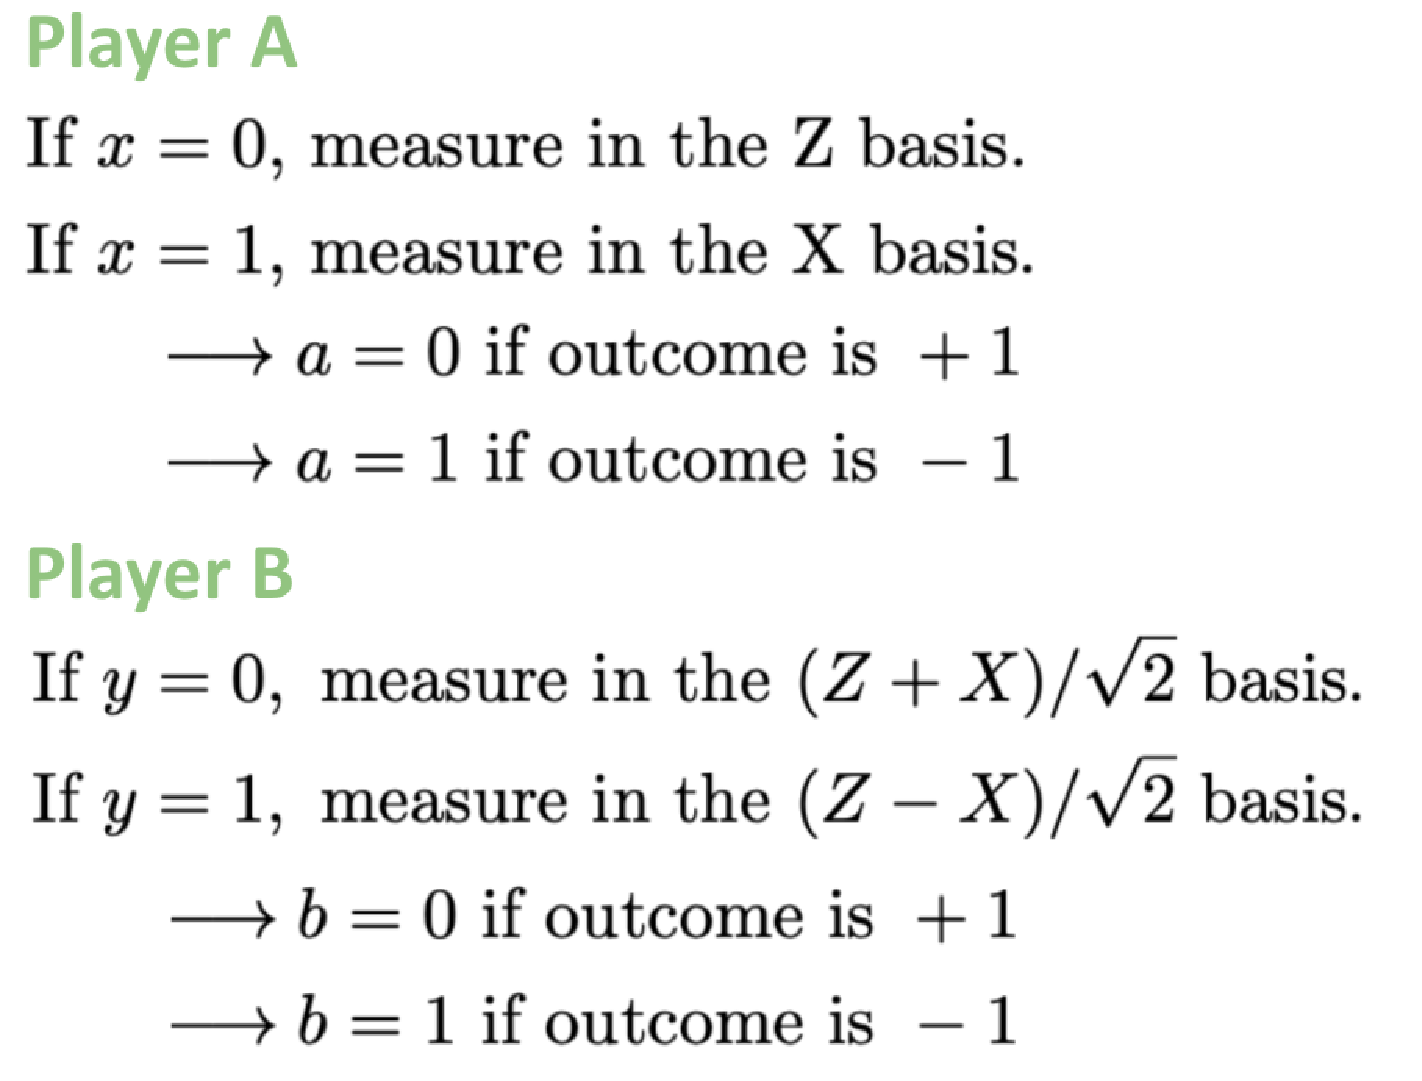
\includegraphics[width=0.8\textwidth]{lesson4/CHSH_quantum_guide.pdf}
        \caption{Summary of quantum version}
    \label{fig:chsh-quantum-summary}
\end{figure}

So far, A and B have used a classical strategy, but what if they implement a quantum strategy, as in Figs.~\ref{fig:chsh-quantum} and \ref{fig:chsh-quantum-summary}? First of all, what \emph{is} a quantum strategy? Well, one strategy is that A and B can share a quantum state, and for concreteness we can assume that the state that they share is 
\begin{equation}
\ket{\psi}_{AB} = \frac{1}{\sqrt2}(\ket{00} + \ket{11}).
\end{equation}
A and B choose to do the following: if A receives $x=0$, then it measures its qubit in the Z basis. If it receives $x=1$, it will measure in the X basis. If the outcome of the measurement (whether Z or X) is $+1$, it sets $a=0$ and replies with this bit. On the other hand, if the measurement outcome is $-1$, then A will reply with $a=1$. B follows a similar strategy, but instead of measuring in the Z or X basis, it measures in a \emph{rotated basis}, choosing $Z+X$ or $Z-X$ if it receives $y=0$ or $y=1$, respectively. Again, it replies with $b=0$ if the measurement outcome is $+1$, and $b=1$ if the measurement outcome is $-1$. If A and B follow this strategy, they can achieve a win rate of 85 percent. That's a 10 percent increase over the best classical strategy.
\rdv{More of the math of this could be a good exercise.}
%We will see later that this state is actually a very special state that we will encounter again and again.

\section{Entangled states}



\if0
\begin{equation}
a_{0} b_{1}=a_{1} b_{0}=0 \quad \longrightarrow a_{0}=0 \quad \text { or } \quad b_{1}=0
\end{equation}
\begin{equation}
\begin{aligned}
\ket{\Phi^{+}}&=\frac{1}{\sqrt{2}}(|00\rangle+|11\rangle) &\left|\Phi^{-}\right\rangle=\frac{1}{\sqrt{2}}(|00\rangle-|11\rangle) \\
\ket{\Psi^{+}}&=\frac{1}{\sqrt{2}}(|01\rangle+|10\rangle) &\left|\Psi^{-}\right\rangle=\frac{1}{\sqrt{2}}(|01\rangle-|10\rangle)
\end{aligned}
\end{equation}
\fi

% Step Two: Entangled States.

Now let's look at \emph{entangled states}.  For this discussion, we will consider a system with two qubits, which we assume are held in two different locations.  We will use the term \emph{local state}\index{local state} to refer to the state of either of two qubits alone, and the term \emph{global state}\index{global state} to refer to the two qubits together -- all of the qubits in our simple system.~\footnote{These terms can easily be extended to discuss more than one qubit in each location.}

We saw in Sec.~\ref{sec:multi-qubit} that in order to describe states of many qubits, we have to use the tensor product. For the case of the two qubits A and B, we have the local state $\ket{\psi}_A$ of the qubit A, and a local state $\ket{\psi}_B$ of qubit B. For concreteness, let's say that they are $\ket{0}$ and $\ket{0}$. In order to write the global state of both qubits, we form the tensor product and we call this state $\ket{\psi}_{AB}$, which in this case is simply $\ket{00}$. We can also consider a different state where A is still in $\ket{0}$ but B is now in the $\ket{+}$ superposition of zero and one. Again, the global state is very simple: form the tensor product of $\ket{0}$ and $\ket{+}$, and when you expand the $\ket{+}$, you can write it in the computational basis, and it's an equal superposition of $\ket{00}$ and $\ket{01}$,
\begin{equation}
\ket{\psi}_{AB} = \ket{0}\ket{+} = \ket{0}\left(\frac{\ket{0} + \ket{1}}{\sqrt{2}}\right) = \frac{\ket{00} + \ket{01}}{\sqrt2}.
\end{equation}
So this is going from local states to global states, but we can also ask the reverse question: given the global state, how do you write the local states of the qubits? In particular, we can consider the following global state which we have encountered in the CHSH game in the previous section,
\begin{equation}
\ket{\psi}_{AB} = \frac{1}{\sqrt2}(\ket{00} + \ket{11})
\end{equation}
which is an equal superposition of $\ket{00}$ and $\ket{11}$.

So what are the local states of qubit A and qubit B? Let's write it out. We can write a general state of qubit A as a superposition of zero and one, with probability amplitudes $a_0$ and $a_1$, and the same for qubit B where the probability amplitude for state zero is $b_0$, and for state one is $b_1$. 
% Just to remind ourselves, 
Let's form a tensor product of $\ket{\psi}_A$ with $\ket{\psi}_B$. We get the following: 
\begin{equation}
\begin{aligned}
|\psi\rangle_{A} \otimes|\psi\rangle_{B} &= \left(a_{0}|0\rangle+a_{1}|1\rangle\right) \otimes\left(b_{0}|0\rangle+b_{1}|1\rangle\right) \\
 &= a_0 b_0\ket{00} + a_0 b_1\ket{01} + a_1 b_0\ket{10} + a_1 b_1\ket{11}.
\end{aligned}
\end{equation}
We get four terms, one probability amplitude for each computational basis term. Let's lay our the mathematical requirements for this equation to match our desired state.
%, we have a-zero b-zero for state $\ket{00}$, a-zero b-one for the state zero-one, a-one b-zero for one-zero, and a-one b-one for $\ket{11}$. 

Remember, the global state that we are looking for is the following: $\ket{00}+\ket{11}$ (normalized appropriately, of course). 
When we compare this general tensor product of A and B with our desired global state and try to determine the values of $a_i$ and $b_i$ we need, we see that
\begin{equation}
a_{0} b_{0}=a_{1} b_{1}=\frac{1}{\sqrt{2}}.
\end{equation}
Okay, so that's requirement number one for our solution.

Requirement number two is that in the global state, we don't have any contributions to the superposition from the $\ket{01}$ and $\ket{10}$ terms,
\begin{equation}
a_0 b_1 = a_1 b_0 = 0.    
\end{equation}

Let's look at the second requirement first. We can see that either $a_0$ must be zero, or $b_1$ must be zero, but if we set either of those to zero and then go back to requirement one, then we see that $a_0 b_0$ or $a_1 b_1$ will also be zero and we will not be able to satisfy requirement one.
%So a-zero cannot be zero. So, we go to b-one equal to zero, and again we see by going back to requirement one that even b-one cannot be equal to zero. 
So did we make a mistake somewhere? In fact, no. It's just a contradiction, and it's just the property of this particular state that we are trying to find local states for. In fact, \emph{not all global states can be written as a tensor product of local states}, and this is the definition of an entangled state.

So we have two major classes of states: first, we have \emph{product states}\index{product state}. % \marginpar{product state}. 
\emph{A product state is one that can be written as a tensor product of local states.} Given some local states $\ket{\psi}_A$ and $\ket{\psi}_B$, we can easily find the global state just by forming the tensor product, and this implies that perfect knowledge of local states implies perfect knowledge of global states.

Second, we have the other class of quantum states which are \emph{entangled states}\index{entangled state}. \emph{An entangled state is a state whose global state cannot be written as the tensor product of local states.} In the previous example, we have demonstrated that for an equal superposition of $\ket{00}$ and $\ket{11}$, this is in fact the case. There are no local kets $\ket{\psi}_A$ and $\ket{\psi}_B$ such that when we take them and form a tensor product, we get the global state back. Mathematically, we can write this as
\begin{equation}
|\psi\rangle_{A B} \neq|\psi\rangle_{A} \otimes|\psi\rangle_{B}.
\end{equation}
This is very interesting because it implies that \emph{we have perfect knowledge of the global state, but we have somehow imperfect knowledge of local states}.

%%%%%%%%%%%%%%%%%%%%%%%%%%%%%%%%%%%%%%%%%%%%%%%
\section{Bell states}

%%%%%%%%%%%%%%%%%%%%%%%%%%%%%%%%%%%%%%%%%%%
\if0
% add all bases having same outcome probabilities
\begin{figure}[H]
    \centering
    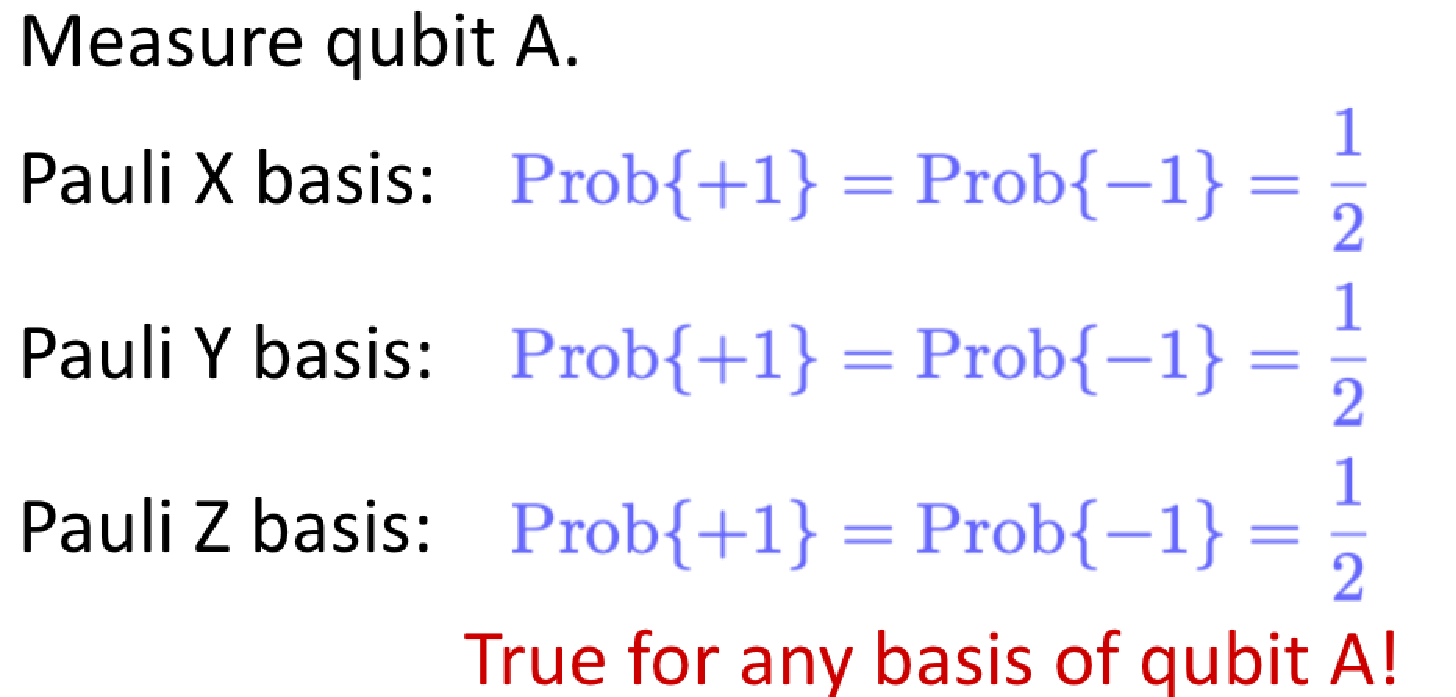
\includegraphics[width=0.8\textwidth]{lesson4/Qubit_A.pdf}
    \label{fig: 1}
    
        \caption{A measurement result}
    
\end{figure}

% B Qubit measurement results
\begin{figure}[H]
    \centering
    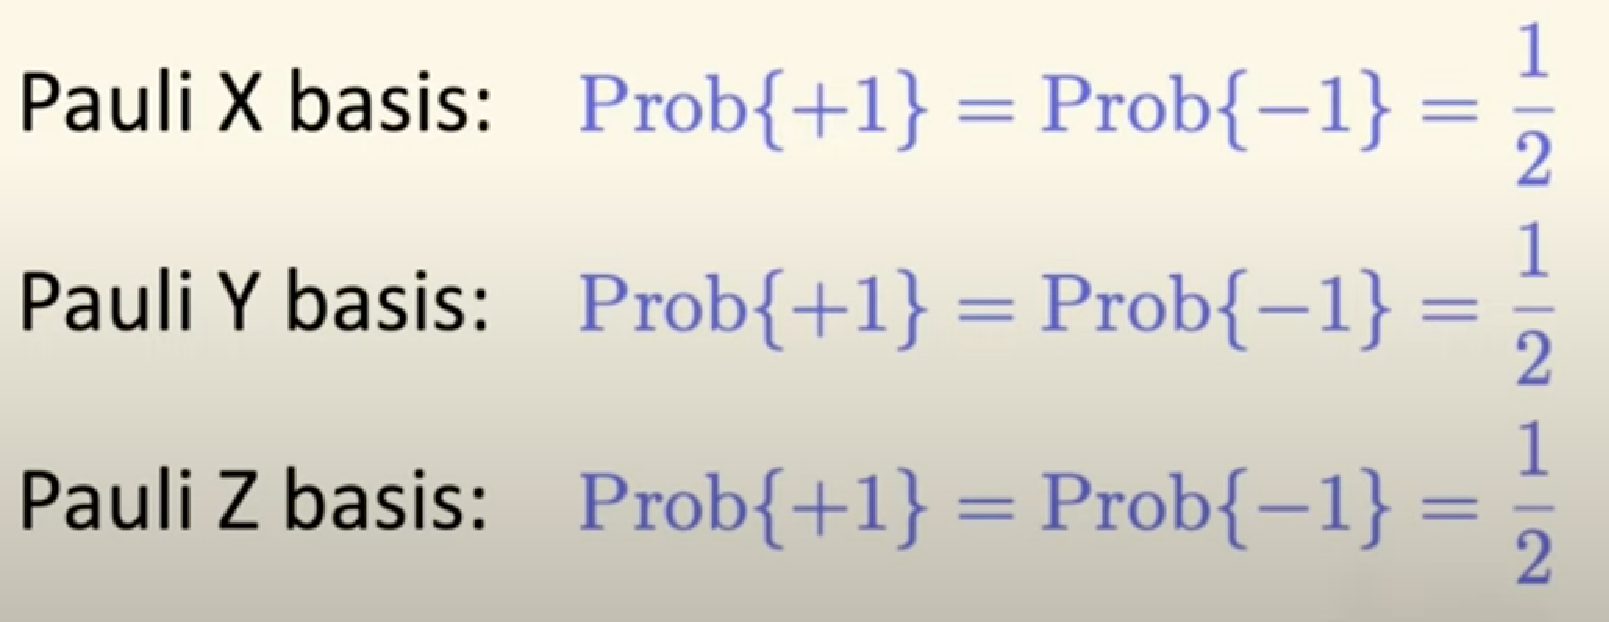
\includegraphics[width=0.8\textwidth]{lesson4/Qubit_B.pdf}
    \label{fig: 1}
    
        \caption{B measurement result}
    
\end{figure}
\fi
%%%%%%%%%%%%%%%%%%%%%%%%%%%%%%%%%%%%%%%%%

\begin{figure}[H]
    \centering
    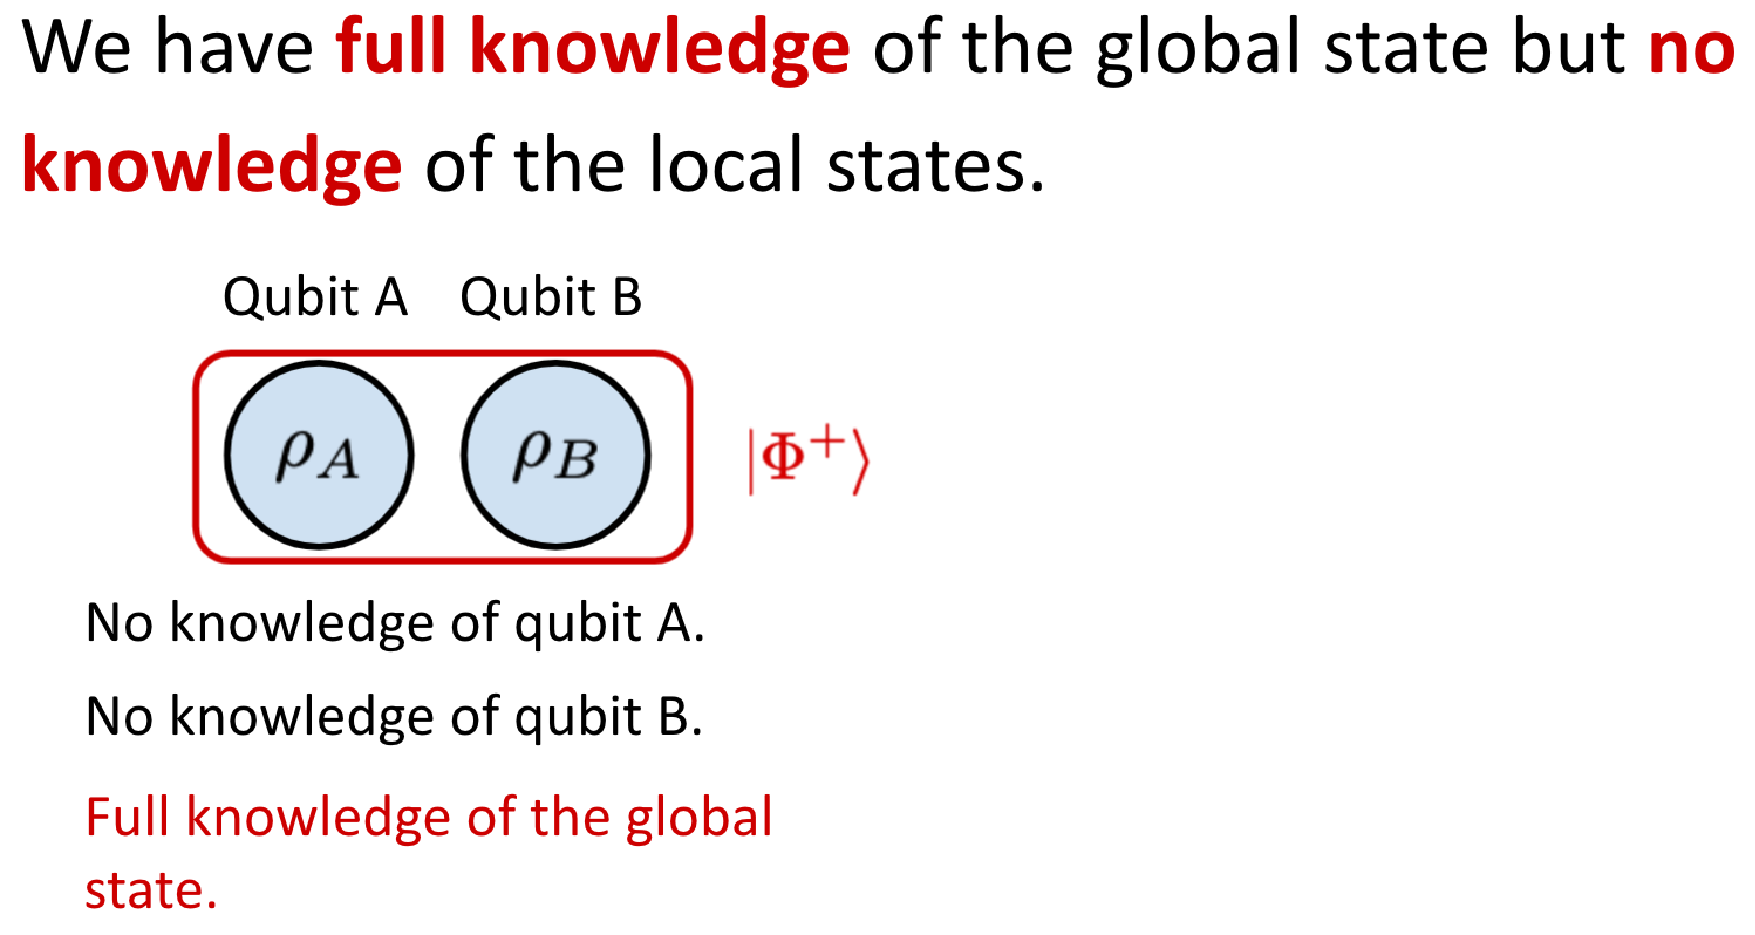
\includegraphics[width=1.0\textwidth]{lesson4/4.3_Recap.pdf}
        \caption[Complete global but no local information]{When entangled states are considered, it is possible to have complete information about the global state but have no information about the local state.}
    \label{fig:incomplete-information}
\end{figure}

%Step Three: Bell States.

We have said that the Bell states\index{Bell states} form a very important class of entangled states of two qubits. There are four of them, and we can write them as follows: 
\begin{equation}
    \begin{aligned}
        |\Phi^+\rangle & = \frac{1}{\sqrt{2}} \left( |00\rangle + |11\rangle \right), & 
        |\Phi^-\rangle = \frac{1}{\sqrt2} \left( |00\rangle - |11\rangle \right), \\
        |\Psi^+\rangle & = \frac{1}{\sqrt{2}} \left( |01\rangle + |10\rangle \right), & 
        |\Psi^-\rangle = \frac{1}{\sqrt2} \left(|01\rangle - |10\rangle \right).
    \end{aligned}
\end{equation}
We have already encountered the equal superposition of $\ket{00}$ plus $\ket{11}$. Normally, we call that a $\ket{\Phi^+}$ (read "phi-plus") state. Its counterpart is the $\ket{\Phi^-}$ ("phi-minus") state, where the $\ket{00}$ and $\ket{11}$ have opposite phase, as shown by the minus sign. There are two more states, $\ket{\Psi^+}$ and $\ket{\Psi^-}$, which are superpositions of \ket{01} and \ket{10}, with \ket{\Psi^-} having opposite phase between the two terms.  These states we will see again and again in the context of quantum communication, quantum computation, quantum key distribution -- basically throughout this entire book and throughout your career in quantum information.~\footnote{In some texts and papers, more commonly but not exclusively older ones, you will see these states written using the lower-case Greek letters $\phi$ (phi) and $\psi$ (psi).  In this book, we will use the capital Greek letters when referring to the Bell pairs and the lower-case letters when referring to specific variables.} 

An interesting thing about the Bell states is that they form an orthogonal basis for two qubits, so we can begin by rewriting the individual vectors for the computational basis in terms of the Bell basis. Just by doing very simple juggling of the terms, you can see that $\ket{00}$ can be written as a superposition of $\ket{\Phi^+}$ and $\ket{\Phi^-}$, and similarly $\ket{01}$ is an equal superposition of $\ket{\Psi^+}$ and $\ket{\Psi^-}$.
All four computational basis states of two qubits can be written in the Bell basis as follows,
\begin{equation}
\begin{aligned}
|00\rangle &=\frac{1}{\sqrt{2}}\left(\left|\Phi^{+}\right\rangle+\left|\Phi^{-}\right\rangle\right), & 
\ket{01} = \frac{1}{\sqrt2}(\ket{\Psi^{+}} + \ket{\Psi^{-}}), \\
|10\rangle &=\frac{1}{\sqrt{2}}\left(\left|\Psi^{+}\right\rangle-\left|\Psi^{-}\right\rangle\right), & 
\ket{11} = \frac{1}{\sqrt2}(\ket{\Phi^{+}} - \ket{\Phi^{-}}).
\end{aligned}
\end{equation}
%, whereas one-zero is an equal superposition of $\ket{\psi^+}$ minus $\ket{\psi^-}$, and $\ket{11}$ is given by phi-plus minus phi-minus. 
This means that we can take any pure state of two qubits given in the form with arbitrary probability amplitudes $\alpha$, $\beta$, $\gamma$, $\delta$,
\begin{equation}
|\psi\rangle=\alpha|00\rangle+\beta|01\rangle+\gamma|10\rangle+\delta|11\rangle
\end{equation}
and we can rewrite it in terms of the Bell states.  Of course the probability amplitudes have to transform accordingly,
%rewriting as in \textbf{Eq. 4.7} and \textbf{4.8},
\begin{equation}
|\psi\rangle=\frac{\alpha+\beta}{\sqrt{2}}\left|\Phi^{+}\right\rangle+\frac{\alpha-\beta}{\sqrt{2}}\left|\Phi^{-}\right\rangle+\frac{\gamma+\delta}{\sqrt{2}}\left|\Psi^{+}\right\rangle+\frac{\gamma-\delta}{\sqrt{2}}\left|\Psi^{-}\right\rangle.
\end{equation}

So this means that now we can even measure in the Bell basis, and we know what probabilities of the various outcomes we get. But remember in the previous chapters we were asking questions: Is the state in zero? Is the state in one? Is the state in plus? Is the state in minus?  This time, we are dealing with two qubits, so there are four possible outcomes. Now the question is: Is the state in $\ket{\Phi^+}$? Is it in $\ket{\Phi^-}$? Is it in $\ket{\Psi^+}$? Or is it in $\ket{\Psi^-}$? These are all the different possible outcomes of the measurement, with probabilities
\begin{equation}
\begin{aligned}
&\operatorname{Prob}\left\{\left|\Phi^{+}\right\rangle\right\}=\frac{|\alpha+\beta|^{2}}{2} \quad \operatorname{Prob}\left\{\left|\Phi^{-}\right\rangle\right\}=\frac{|\alpha-\beta|^{2}}{2} \\
&\operatorname{Prob}\left\{\left|\Psi^{+}\right\rangle\right\}=\frac{|\gamma+\delta|^{2}}{2} \quad \operatorname{Prob}\left\{\left|\Psi^{-}\right\rangle\right\}=\frac{|\gamma-\delta|^{2}}{2}
\end{aligned}
\end{equation}
Because we already rewrote the state $\ket{\psi}$ in the Bell basis, it's very easy to read out the probabilities of measurement outcomes.
This will be again very important because measurements in the Bell basis are crucial in many protocols in quantum communication, especially teleportation and entanglement swapping, which we will look at quite closely later in this book.

Let's ask a different question: If we are sharing a \ket{\Phi^+} Bell pair, if we measure in the Bell basis, we will find the state \ket{\Phi^+} with 100\% probability. But what happens if we measure just one qubit of the pair? Remember that we encountered this scenario in the CHSH game, where the players were sharing a Bell state, and they performed local measurements on the qubits that were in their possession. 
%So let's take as a concrete example the state $\ket{\Phi^+}$, as we saw in the CHSH game. 
If we measure only qubit A in the Z basis and leave qubit B untouched, we can compute the probabilities of the $+1$ outcome and the $-1$ outcome and find that they are an equal one-half. \rdv{Go through this derivation.}  We can go through the same thing for measuring qubit B, and again we see the same behavior.

\label{page:plus-is-pure}
At this point, you may be a little puzzled; didn't we see this same fifty-fifty behavior with a single qubit in the $\ket{+}$ state?  What is different with entanglement?  When measuring in the Z basis, it is true that we always see the fifty-fifty statistics.  However, if we measure a $\ket{+}$ in the X basis, we will \emph{always} find that the state is in the $+1$ state.  We can also choose to apply a Hadamard gate to the $\ket{+}$ state and return it to a known $\ket{0}$ state.  Thus, although the qubit is in superposition, we have complete information about that superposition.  In contrast, when we hold only one qubit of an entangled pair and attempt to measure it, our results will differ.

%\rdv{This par fails to completely close the deal in demonstrating that we don't have any local information, since the outcomes are 50/50 both when we are talking about a single plus state and a Bell state.  Needs a counterpoint where we have full information?  Show that the single plus state always has a specific outcome when measuring in the X basis.} Added above.

If we change the measurement basis to a Pauli Y basis, again we find that the probability of the $+1$ outcome is the same as the probability of the $-1$ outcome. It is the same for the X basis, and in fact in any basis that you measure qubit A, you will get the same result: both outcomes are fifty-fifty. In fact, the local measurement results are uniformly random in any basis. Remember the state of the global system is pure. We know exactly what it is, yet no matter in what basis we measure the states locally we are getting 50 percent one outcome and 50 percent the other outcome. We can say that we have no knowledge of the local states of qubit A and qubit B. This goes back to our previous discussion about the difference between entangled states and product states.  Since this state is entangled, the correct description of the local qubits must be given in terms of density matrices, and we can write that the state of qubit A is a maximally mixed state. With probability half it's in the zero state, and with probability half it's in the one state. The same holds for qubit B. Again we write it as a maximally mixed state,
\begin{equation}
\begin{aligned}
&\rho_A=\frac{1}{2}(|0\rangle\langle 0|+| 1\rangle\langle 1|) \\
&\rho_B=\frac{1}{2}(|0\rangle\langle 0|+| 1\rangle\langle 1|).
\end{aligned}
\end{equation}

Just to stress how strange this is that we have a full knowledge of the global state yet we have zero knowledge of the local states, let's look at this again: qubit A is a maximally mixed state. We have no knowledge about its state. The same is true for qubit B considered in isolation. Yet, somehow, when we look at the state globally, we have perfect knowledge of the entire state. This distinction is addressed more in the chapter exercises.


%%%%%%%%%%%%%%%%%%%%%%%%%%%%%%%%%%%%%%%%%%%%%%%%%%%%%%%%%
\section{SPDC}
\label{sec:4-4_spdc}

% pic
\begin{figure}[H]
    \centering
    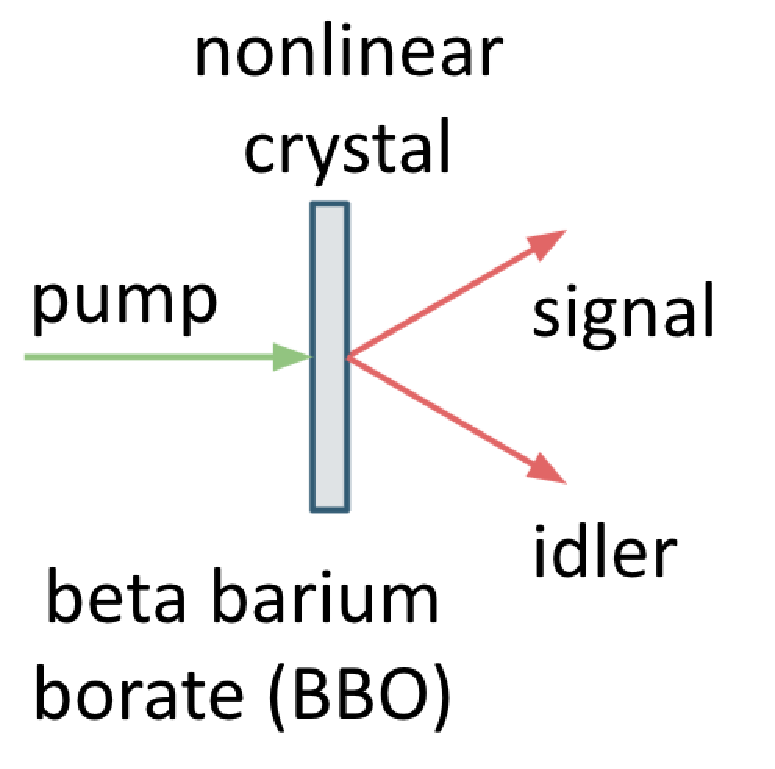
\includegraphics[width=0.5\textwidth]{lesson4/pump.pdf}
    
        \caption[Symmetric parametric down conversion (SPDC)]{Symmetric parametric down conversion (SPDC) turns one high-energy pump photon into two lower-energy entangled photons, with some very low probability. The two output photons are called \emph{signal} and \emph{idler}.}
    \label{fig:spdc}
    
\end{figure}

\begin{figure}[H]
    \centering
    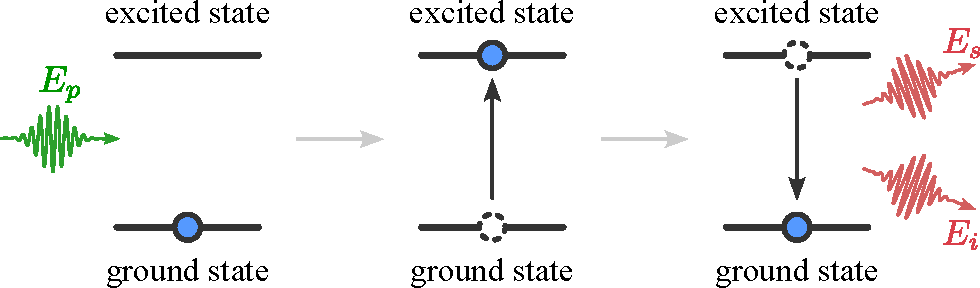
\includegraphics[width=0.8\textwidth]{lesson4/4-8_spdc.pdf}
    
        \caption[pump photon and the energy levels of the atom]{A representation of the pump photon of energy $E_p$ and the energy levels of the atom. Energy level diagrams such as these are an abstraction that allows us to describe absorption and emission of photons by an atom. The circle indicates that there is a single electron in the ground state.
        The atom absorbs the energy provided by the pump photon and transitions to the excited state. The atom decays spontaneously after some time, releasing energy in the form of two photons with energies $E_s$ and $E_i$. Due to conservation of energy, we have $E_p = E_s + E_i$.}
    
    \label{fig:spdc-energy-levels}
\end{figure}

% \begin{figure}[H]
%   \centering
%   \begin{minipage}[b]{0.3\textwidth}
%     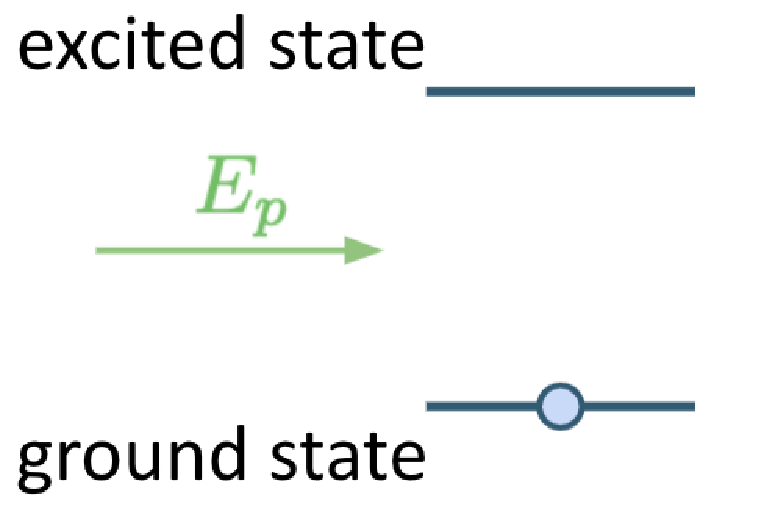
\includegraphics[width=\textwidth]{lesson4/state1.pdf}
%     \caption{A representation of the pump photon and the energy levels of the atom.}
%   \end{minipage}
%   \hfill
%   \begin{minipage}[b]{0.3\textwidth}
%     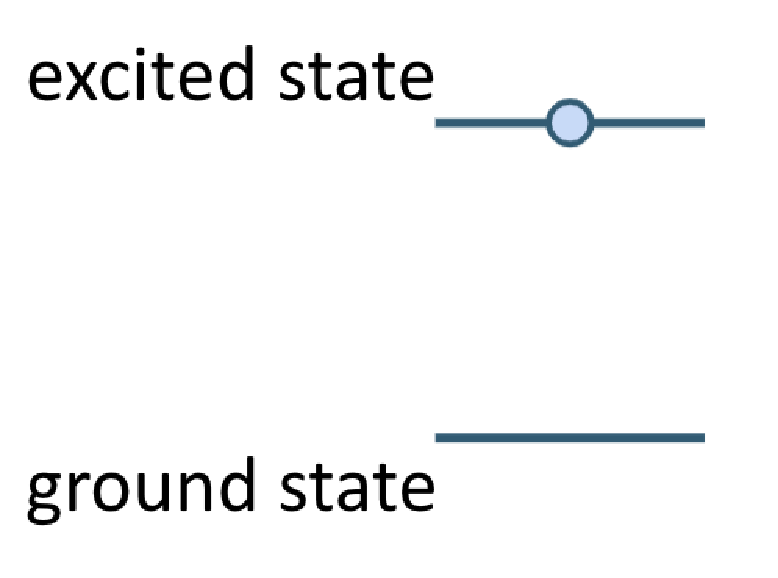
\includegraphics[width=\textwidth]{lesson4/state2.pdf}
%     \caption{After absorption of the photon, the electron moves to the excited state.}
%   \end{minipage}
%   \hfill
%   \begin{minipage}[b]{0.3\textwidth}
%     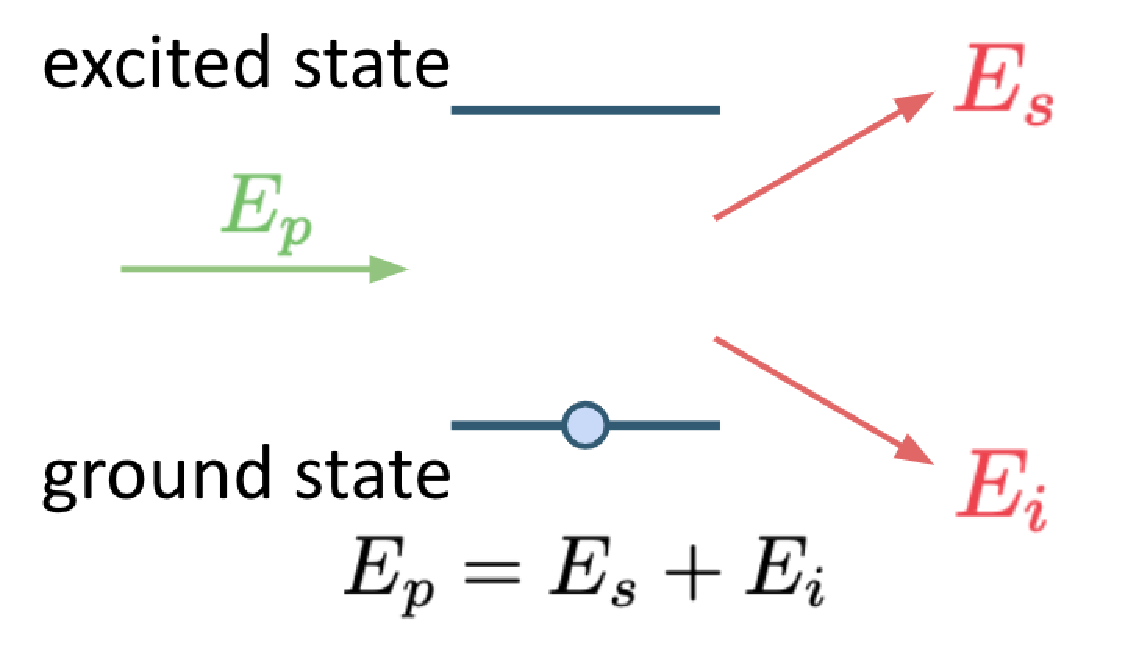
\includegraphics[width=\textwidth]{lesson4/state3.pdf}
%     \caption{A representation of the emission of two photons when the electron decays from the excited state back to the ground state.}
%   \end{minipage}
% \end{figure}

\begin{figure}[H]
    \centering
    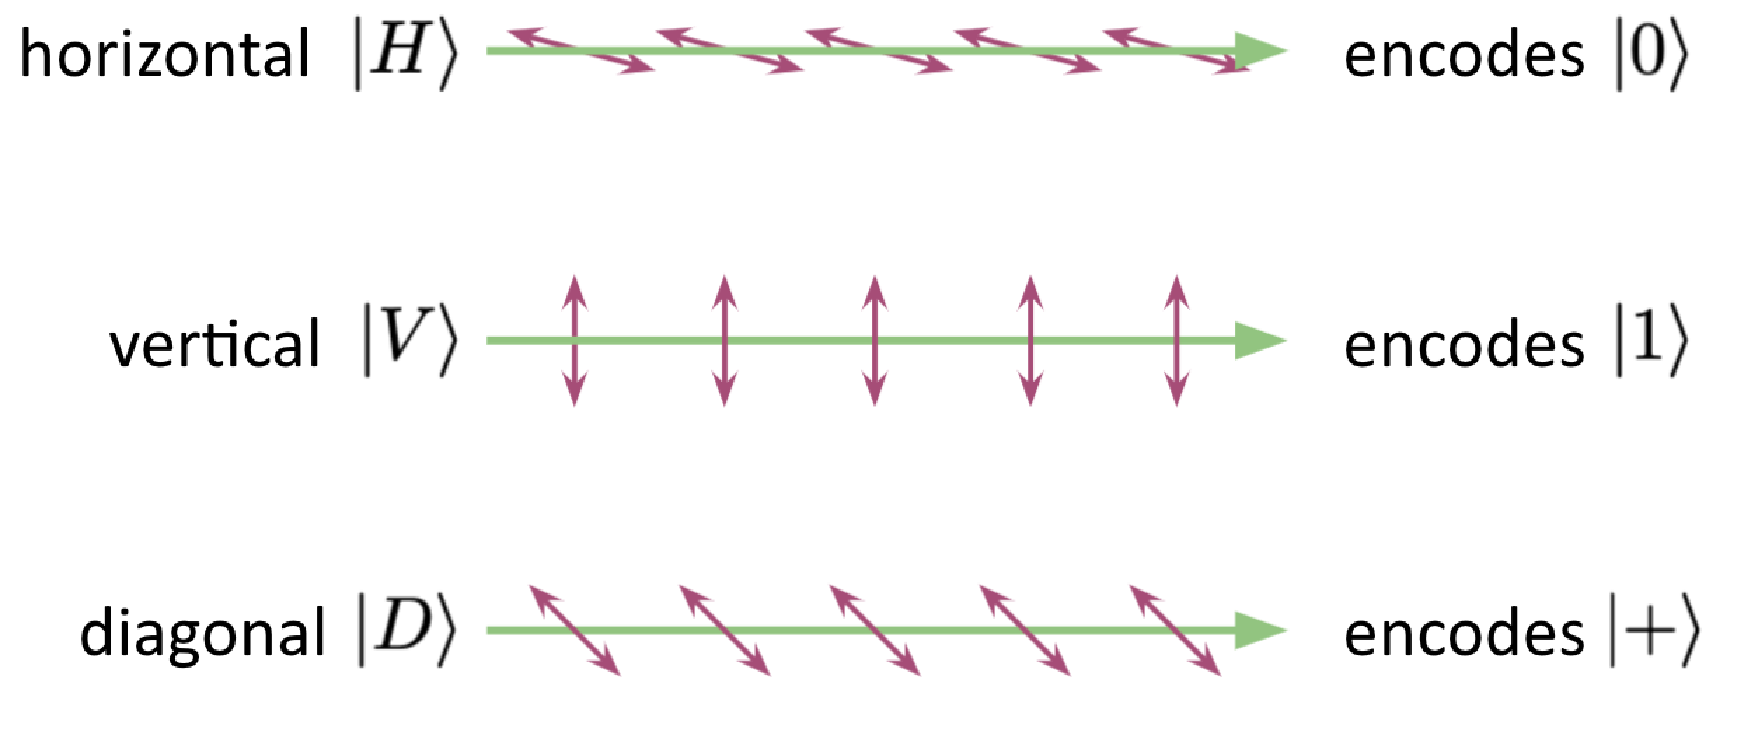
\includegraphics[width=0.8\textwidth]{lesson4/linear_polarization.pdf}
    
        \caption[Horizontally, vertically and diagonally polarized light]{If horizontally and vertically polarized light are used to encode $\ket{0}$ and $\ket{1}$, then diagonally polarized light encodes $\ket{+}$.}
    
    \label{fig:hvd-light}
\end{figure}

\begin{figure}[H]
    \centering
    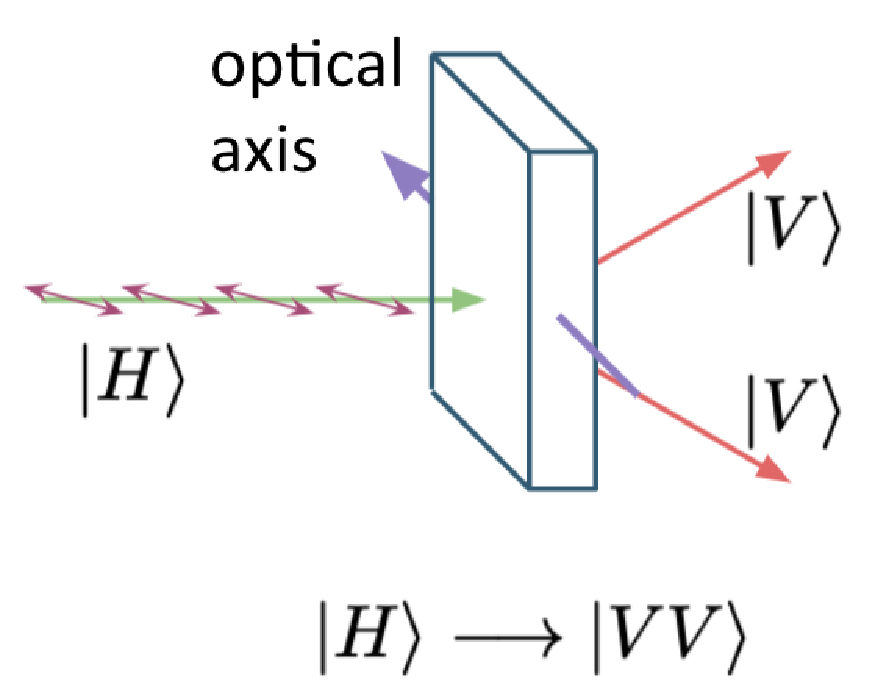
\includegraphics[width=0.5\textwidth]{lesson4/horizontal_optical_axis.pdf}
    
        \caption{Horizontally polarized light matching the optical axis of the crystal can be down-converted to vertically polarized pairs of photons.}
    
    \label{fig:horizontal-opt-axis}
\end{figure}

\begin{figure}[H]
   \centering
    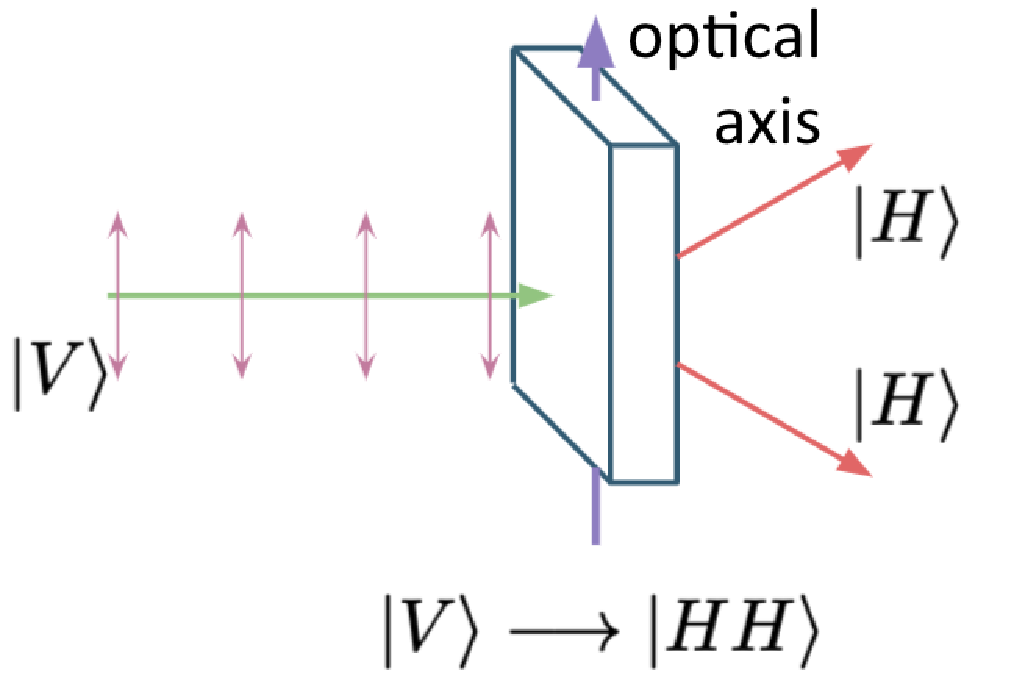
\includegraphics[width=0.5\textwidth]{lesson4/vertical_optical_axis.pdf}
    
        \caption{Vertically polarized light matching the optical axis of the crystal can be down-converted to horizontally polarized pairs of photons.}
    
    \label{fig:vertical-opt-axis}
\end{figure}

% Step Four: SPDC.

In this section, we will learn how to actually generate entangled states physically. Specifically, we will look at the process of \emph{spontaneous parametric down-conversion}\index{spontaneous parametric down-conversion (SPDC)}, or SPDC for short. There are many physical processes that can generate entangled pairs of photons, but this one is  common in laboratories and will serve as our example. \rdv{Soon suggests explaining each word separately.} \rdv{“spontaneous” means that the process is not stimulated.
In a spontaneous process, no other input is needed, only the incoming photon of high energy that gets converted into two photons of lower energies.
In a stimulated process you need the input photon and some other photon as well. A good example would be lasing. “parametric” means the whole process does not depend only on the intensity of the electric field but also on the phase of the field. “parametric” in the context of SPDC means there is a relationship between the input and output electric fields.}

We will demonstrate SPDC with the little graphic in Fig.~\ref{fig:spdc}. Imagine that you have some laser light, represented by the green arrow, which we call the \emph{pump}, incident normally on a non-linear crystal represented by the rectangle. In this particular case, we are using a beta barium borate, or BBO, crystal, which is a popular choice in experiments. This pump laser gets transformed and split into two beams. One beam is called the "signal" and the other one is called the "idler". If we actually zoom into the crystal to see what happens to individual atoms, we get the following picture: the pump light is tuned to be resonant with some transition frequency of the atoms inside the BBO crystal, so to a good approximation it affects only two levels. The lower level we will call the "ground state" and the upper level we will call the "excited state". The atom in the BBO crystal starts in the ground state, but then it gets blasted by this pump laser.  The atom becomes excited and absorbs the energy from the incoming pump laser, and after a short time the atom de-excites and ejects two photons with energy $E_s$ for the signal photon and energy $E_i$ for the idler photon.   \rdv{Why two instead of one?}  Because energy is conserved in this transition, we must have that the energy of the pump photon must be equal to the sum of the energies of the outgoing photons, $E_p = E_s + E_i$. This is the basic process of spontaneous parametric down-conversion.

Now let's see how polarization of light interacts with this process. Consider linearly polarized light. If we again take our green pump laser, we can make it oscillate only in one plane. For example, if we make it oscillate in the horizontal plane, this can encode our $\ket{0}$ state of a qubit, as in Fig.~\ref{fig:hvd-light}. We can also make the light oscillate only in the vertical plane, in that case we will say that this encodes a $\ket{1}$. We already know from previous sections and chapters that we can talk about superpositions of these states. When we go to the polarization picture, we can get diagonally polarized light which we call \ket{D}, and this will encode our equal superposition of $\ket{0}$ and $\ket{1}$, or as we call it a $\ket{+}$ state. That's the next ingredient that we're going to need in producing entangled pairs of photons.

How does polarized light actually interact with this nonlinear BBO crystal? That depends on the optical axis of the crystal. For now, we don't have to worry too much about what an optical axis is and how it's defined. Just remember that there is some kind of special direction in which the BBO crystal can be aligned and that's very important relative to the incoming light and its polarization. If the optical axis aligns horizontally, and the incoming light is horizontally polarized, then the photons that are coming out from the crystal (the signal and the idler) will both be vertically polarized. So this setup, as shown in Fig.~\ref{fig:horizontal-opt-axis} -- horizontally polarized pump light and optical axis in the direction represented by the purple arrow -- implements the physical transformation
\begin{equation}
\begin{aligned}
\ket{H} &\rightarrow \ket{VV}.
\end{aligned}
\end{equation}
It takes a horizontally polarized state and it outputs two vertically polarized states.

On the other hand, we can also rotate the optical axis of the BBO crystal, as in Fig.~\ref{fig:vertical-opt-axis} and in this case if we have a vertically polarized light incident on the BBO crystal, then the two photons will both be horizontally polarized.  In this case we are implementing the physical transformation
\begin{equation}
\begin{aligned}
\ket{V} &\rightarrow \ket{HH}.
\end{aligned}
\end{equation}

\rdv{what happens if the light and the optical axis are orthogonal? Nothing?}

% What we can do is we can, in fact- and just so that it's clear the polarization of the photon pairs is always opposite to the one to the polarization of the pump- so next, what we can do is
We have one last step that we actually need to produce entangled photon pairs.  We take two of these BBO crystals and put them next to each other, and arrange them such that their optical axes will be orthogonal to each other.

In such a geometry, when we set the pump laser to be diagonally polarized, we get the following transformation: diagonally polarized light will become a superposition of the horizontally polarized photons and vertically polarized photons,
\begin{equation}
    \ket{D} \rightarrow \frac{\ket{HH}+\ket{VV}}{\sqrt{2}}.
\end{equation}
You can see that we are changing a $\ket{+}$ state into a Bell pair $(\ket{00}+\ket{11})/\sqrt{2}$, and this is in fact how we get entangled states using SPDC.  In order for this to work, the BBO crystals have to be very, very thin. This will ensure that we are not quite sure whether the photons were produced in the first crystal or in the second crystal. We call this the \emph{indistinguishability criterion}, and if this is satisfied then we can talk about genuinely entangled photons. If, however, we can actually tell where the two photons originate, then we will only get horizontally polarized photons or we will get vertically polarized photons, and there will be no entanglement shared between these two photons. 

Another important property of SPDC is that it's an extremely rare process.  We obtain only about one photon pair per $10^6$ pump photons, and even that level is achieved only in state-of-the-art experiments. In a more common laboratory setup, it takes several orders of magnitude more pump photons to successfully create each entangled pair.  The photons that are not down-converted simply pass through the crystal unaffected and are discarded.

There are many details around SPDC that we have not introduced here, but this basic understanding is adequate for our purposes in this book.

% Usually this number- this ten-to-the-six pump photons is much higher or orders of magnitudes higher in commercially available lasers.


%%%%%%%%%%%%%%%%%%%%%%%%%%%%%%%%%%%%%%%%%%%%%%%%
\section{Entanglement as a resource}

% insert broken connection 
\begin{figure}[H]
   \centering
    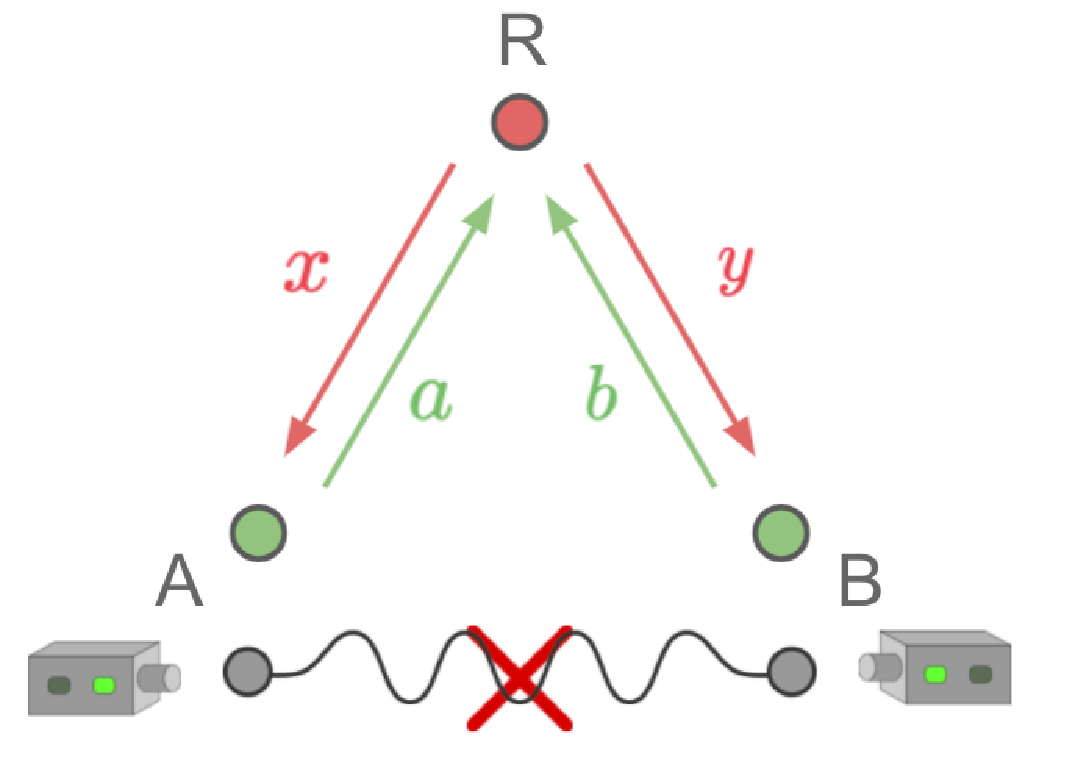
\includegraphics[width=0.8\textwidth]{lesson4/CHSH_broken_entanglement.pdf}
    
        \caption{In the CHSH game, each time the players play, they collapse (break) one entangled state.}
    
    \label{fig:chsh-broken}
\end{figure}

% Step Five: Entanglement as a Resource.

Let's go back and revisit our CHSH game from the first section of this chapter. We have seen that entanglement can actually help players A and B win the game more often. If they share an entangled state, they can perform measurements on it and this will help them in winning the game with higher probability. But in this process of measurement, as shown in Fig.~\ref{fig:chsh-broken}, A and B destroy the entanglement shared between the two grey qubits.  Maybe they managed to win the game, at least this particular round, but if they want to win again, they have to find a way of re-establishing this entanglement or creating a new entangled pair which they can share and then use in the new round of the game. 

Entanglement is also crucial in quantum networks.
Figure~\ref{fig:4-5_resource_network} shows a simple quantum network, where the blue circles represent the network nodes.
They could be individual qubits or even small quantum computers, for now the distinction is not important.
The lines joining the network nodes represent shared entanglement.
There is a sender node in possession of a qubit, represented by the red circle, that it is trying to communicate to the receiver node.
Usual way of sending quantum information is to use the teleportation protocol, which we will discuss in detail in Chapter~\ref{sec:8_teleportation}.
For now, all we need to know is that the protocol consumes a single Bell pair to transfer the quantum information from one node to its neighboring one.
By executing the teleportation protocol first at the sender's node, and then at nodes $N_1$ and $N_2$, the quantum information will be delivered to the receiver node.
We can see that delivering the quantum information has consumed all the entangled pairs along the path connecting the sender with the receiver.
In order for the quantum network to be fully functional again, we must re-establish the destroyed entangled links.

\begin{figure}[t]
    \centering
    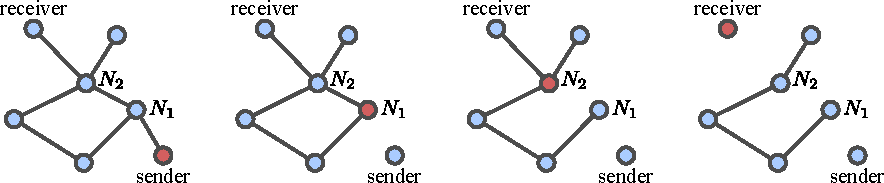
\includegraphics[width=\textwidth]{lesson4/4-5_resource_network.pdf}
    \caption[Consumption of entanglement in a quantum network.]{Entanglement is consumed as quantum information is propagated from the sender to the receiver.}
    \label{fig:4-5_resource_network}
\end{figure}

We can think of entanglement as the fuel that drives many quantum technologies. Entanglement offers improved, and sometimes completely new, functionality that is not seen in either classical networks or classical computation.
One of the key takeaways is that entanglement is a \textbf{\textit{resource}}, and is consumed just like fuel in your car or battery charge in your phone.
It is the job of quantum networks to distribute entanglement in order to satisfy the demand for this precious resource.


\newpage
\begin{exercises}
\exer{Prove that the four Bell states are orthogonal to each other.}

\exer{\rdv{Find the probabilities of the different measurement outcomes for several states.}}

\exer{On p.~\pageref{page:plus-is-pure}, we stated without proof that measuring the state of a single qubit in $\ket{+}$ provides different outcome statistics than measuring one qubit that is part of a Bell pair.  Prove this by calculating the outcome probabilities for measuring both the single qubit and the half of the Bell pair, when using the X, Y, and Z measurement bases.  (Hint: this problem will be easier if you have done the problems in Ch. 3.)}

\exer{\rdv{Do some rough calculations of number of entangled photon pairs output for a certain wattage of laser, wavelength, and conversion efficiency.}}

\exer{\rdv{Two-qubit measurement exercises.}}
\end{exercises}


\newpage
\section*{Quiz}
  \addcontentsline{toc}{section}{Quiz}

% \section{Learning more}

The online version of this course includes a quiz for this block of chapters. Discussion of the quiz questions will be provided there.

\section*{Further reading for chapters 1-4}
  \addcontentsline{toc}{section}{Further reading for chapters 1-4}

{\bf chapter 1}\\

The first chapter serves as a gentle introduction to the area of quantum communication. Its goal is to provide a qualitative overview and discuss ideas behind communication and its evolution rather than focusing on any quantitative discussion.

An excellent popular science book on this topic is James Gleick, \emph{The Information: A History, The Theory, A Flood}~\cite{gleick2012information}. It covers the evolution of communication and spends a sizeable portion of its length on discussing the switch from analog to digital. However, it does not cover quantum communication.

There are also a number of great science YouTube channels with excellent, concise introductions on the topic of quantum communication and computation:
\begin{enumerate}
    \item Veritasium
    \item Science Girl
    \item PBS Space Time
\end{enumerate}

{\bf chapter 2}\\

The second chapter is a lot more technical and introduces fundamental concepts such as qubits and measurements, which we will encounter throughout the entire curriculum. Being comfortable with these concepts and knowing how to describe them mathematically is crucial.

An article by Perry \emph{et al.} called "Quantum Computing as a High School Module" is a great extension to the content of this and following chapters. It introduces basic mathematical descriptions and contains many short exercises designed to check your understanding.

A more advanced introduction to the mathematical concepts in this chapter can be found in the classic textbook by Michael A. Nielsen and Isaac L. Chuang, \emph{Quantum Computation and Quantum Information}~\cite{nielsen-chuang:qci}. Almost all serious quantum researchers have a copy of this book, but its learning curve is steep and we recommend attacking it after a more introductory book or course (which you presumably are gaining through this learning module and other courses). This book, known as "Mike and Ike", covers key ideas in computer science theory, the basic quantum information ideas and algorithms, and the principles of quantum hardware. Its descriptions of hardware and error correction are now rather out of date, and the description of algorithms is limited to a few important cases, but the principles are foundational and the explanation clear.

An alternative to Mike and Ike is John Preskill's lecture notes, which are available chapter by chapter as open access PDF files~\cite{preskill:PH-CS219}.

A new textbook that covers the basics of quantum information and their role in quantum computation and communication is Robert Sutor's \emph{Dancing with Qubits}~\cite{sutor19:dancing}. This textbook spends great effort in explaining the basics and goes over the fundamental calculations in great detail. The first half of the book covers the basic mathematics you will need, including complex numbers, probability and linear algebra (vectors and matrices). We strongly recommend this book for all beginning students, especially those who are worried about the math required. We recommend it to our own beginning undergraduates.

An alternative to Sutor that focuses primarily on basic algorithms is Eleanor Rieffel and Wolfgang Polak's \emph{Quantum Computing: a Gentle Introduction}~\cite{rieffel2011quantum}.

{\bf chapter 3}\\

The third chapter continues with our exposition of the basic mathematical formalism underpinning quantum communication as well as quantum computation. The primary focus is description of noisy quantum states using density matrices.

Chapter 2 of “Mike \& Ike” and Perry’s article mentioned above are great for this chapter as well. Another fantastic book on quantum information (though primarily targeted at graduate students so parts of it might be too technical to follow) is Mark Wilde's \emph{Quantum Information Theory}~\cite{wilde2013quantum}.

Chapter 3 of Wilde’s textbook deals with noisy states. Discussion on fidelity of quantum states can be found in Chapter 9 of “Mike \& Ike” and in Chapter 9 of Wilde’s textbook.

{\bf chapter 4}\\

This chapter is the conclusion of the introductory Block and deals with the scenario when we have multiple qubits which naturally leads to entanglement. Perry’s article, “Mike \& Ike” as well as Wilde’s textbook remain great introductions and ordered in this way represent the ramping up difficulty of mathematical rigour. 

The CHSH game is discussed in Chapter 3 of Wilde’s textbook~\cite{wilde2013quantum}. Another excellent exposition of this game is by Umesh Vazirani as part of his lecture series on YouTube.

A great introduction to SPDC can be found in Betchart’s bachelor's thesis~\footnote{\url{https://etd.ohiolink.edu/apexprod/rws_olink/r/1501/10?clear=10&p10_accession_num=oberlin1206296667}}.

